% This is the Reed College LaTeX thesis template. Most of the work
% for the document class was done by Sam Noble (SN), as well as this
% template. Later comments etc. by Ben Salzberg (BTS). Additional
% restructuring and APA support by Jess Youngberg (JY).
% Your comments and suggestions are more than welcome; please email
% them to cus@reed.edu
%
% See https://www.reed.edu/cis/help/LaTeX/index.html for help. There are a
% great bunch of help pages there, with notes on
% getting started, bibtex, etc. Go there and read it if you're not
% already familiar with LaTeX.
%
% Any line that starts with a percent symbol is a comment.
% They won't show up in the document, and are useful for notes
% to yourself and explaining commands.
% Commenting also removes a line from the document;
% very handy for troubleshooting problems. -BTS

% As far as I know, this follows the requirements laid out in
% the 2002-2003 Senior Handbook. Ask a librarian to check the
% document before binding. -SN

%%
%% Preamble
%%
% \documentclass{<something>} must begin each LaTeX document
\documentclass[12pt,twoside]{templates/facsothesis}
% Packages are extensions to the basic LaTeX functions. Whatever you
% want to typeset, there is probably a package out there for it.
% Chemistry (chemtex), screenplays, you name it.
% Check out CTAN to see: https://www.ctan.org/
%%
\ifxetex
  \usepackage{polyglossia}
  \setmainlanguage{spanish}
  % Tabla en lugar de cuadro
  \gappto\captionsspanish{\renewcommand{\tablename}{Tabla}
          \renewcommand{\listtablename}{Índice de tablas}}
\else
  \usepackage[spanish,es-tabla]{babel}
\fi
%\usepackage[spanish]{babel}
\usepackage{graphicx,latexsym}
\usepackage{amsmath}
\usepackage{amssymb,amsthm}
\usepackage{longtable,booktabs,setspace}
\usepackage{chemarr} %% Useful for one reaction arrow, useless if you're not a chem major
\usepackage[hyphens]{url}
% Added by CII
%\usepackage{hyperref}
\usepackage[colorlinks = true,
            linkcolor = blue,
            urlcolor  = blue,
            citecolor = blue,
            anchorcolor = blue]{hyperref}
\usepackage{lmodern}
\usepackage{float}
\floatplacement{figure}{H}
% End of CII addition
\usepackage{rotating}
\usepackage{placeins} % para fijar la posición de las tablas con \FloatBarrier


\usepackage[]{natbib}


% Next line commented out by CII
%\usepackage{biblatex}
%\usepackage{natbib}
% Comment out the natbib line above and uncomment the following two lines to use the new
% biblatex-chicago style, for Chicago A. Also make some changes at the end where the
% bibliography is included.
%\usepackage{biblatex-chicago}
%\bibliography{thesis}


% Added by CII (Thanks, Hadley!)
% Use ref for internal links
\renewcommand{\hyperref}[2][???]{\autoref{#1}}
\def\chapterautorefname{Chapter}
\def\sectionautorefname{Section}
\def\subsectionautorefname{Subsection}
% End of CII addition

% Added by CII
\usepackage{caption}
\captionsetup{width=5in}
% End of CII addition

% \usepackage{times} % other fonts are available like times, bookman, charter, palatino

% Syntax highlighting #22
  \usepackage{color}
  \usepackage{fancyvrb}
  \newcommand{\VerbBar}{|}
  \newcommand{\VERB}{\Verb[commandchars=\\\{\}]}
  \DefineVerbatimEnvironment{Highlighting}{Verbatim}{commandchars=\\\{\}}
  % Add ',fontsize=\small' for more characters per line
  \usepackage{framed}
  \definecolor{shadecolor}{RGB}{248,248,248}
  \newenvironment{Shaded}{\begin{snugshade}}{\end{snugshade}}
  \newcommand{\AlertTok}[1]{\textcolor[rgb]{0.94,0.16,0.16}{#1}}
  \newcommand{\AnnotationTok}[1]{\textcolor[rgb]{0.56,0.35,0.01}{\textbf{\textit{#1}}}}
  \newcommand{\AttributeTok}[1]{\textcolor[rgb]{0.77,0.63,0.00}{#1}}
  \newcommand{\BaseNTok}[1]{\textcolor[rgb]{0.00,0.00,0.81}{#1}}
  \newcommand{\BuiltInTok}[1]{#1}
  \newcommand{\CharTok}[1]{\textcolor[rgb]{0.31,0.60,0.02}{#1}}
  \newcommand{\CommentTok}[1]{\textcolor[rgb]{0.56,0.35,0.01}{\textit{#1}}}
  \newcommand{\CommentVarTok}[1]{\textcolor[rgb]{0.56,0.35,0.01}{\textbf{\textit{#1}}}}
  \newcommand{\ConstantTok}[1]{\textcolor[rgb]{0.00,0.00,0.00}{#1}}
  \newcommand{\ControlFlowTok}[1]{\textcolor[rgb]{0.13,0.29,0.53}{\textbf{#1}}}
  \newcommand{\DataTypeTok}[1]{\textcolor[rgb]{0.13,0.29,0.53}{#1}}
  \newcommand{\DecValTok}[1]{\textcolor[rgb]{0.00,0.00,0.81}{#1}}
  \newcommand{\DocumentationTok}[1]{\textcolor[rgb]{0.56,0.35,0.01}{\textbf{\textit{#1}}}}
  \newcommand{\ErrorTok}[1]{\textcolor[rgb]{0.64,0.00,0.00}{\textbf{#1}}}
  \newcommand{\ExtensionTok}[1]{#1}
  \newcommand{\FloatTok}[1]{\textcolor[rgb]{0.00,0.00,0.81}{#1}}
  \newcommand{\FunctionTok}[1]{\textcolor[rgb]{0.00,0.00,0.00}{#1}}
  \newcommand{\ImportTok}[1]{#1}
  \newcommand{\InformationTok}[1]{\textcolor[rgb]{0.56,0.35,0.01}{\textbf{\textit{#1}}}}
  \newcommand{\KeywordTok}[1]{\textcolor[rgb]{0.13,0.29,0.53}{\textbf{#1}}}
  \newcommand{\NormalTok}[1]{#1}
  \newcommand{\OperatorTok}[1]{\textcolor[rgb]{0.81,0.36,0.00}{\textbf{#1}}}
  \newcommand{\OtherTok}[1]{\textcolor[rgb]{0.56,0.35,0.01}{#1}}
  \newcommand{\PreprocessorTok}[1]{\textcolor[rgb]{0.56,0.35,0.01}{\textit{#1}}}
  \newcommand{\RegionMarkerTok}[1]{#1}
  \newcommand{\SpecialCharTok}[1]{\textcolor[rgb]{0.00,0.00,0.00}{#1}}
  \newcommand{\SpecialStringTok}[1]{\textcolor[rgb]{0.31,0.60,0.02}{#1}}
  \newcommand{\StringTok}[1]{\textcolor[rgb]{0.31,0.60,0.02}{#1}}
  \newcommand{\VariableTok}[1]{\textcolor[rgb]{0.00,0.00,0.00}{#1}}
  \newcommand{\VerbatimStringTok}[1]{\textcolor[rgb]{0.31,0.60,0.02}{#1}}
  \newcommand{\WarningTok}[1]{\textcolor[rgb]{0.56,0.35,0.01}{\textbf{\textit{#1}}}}

% To pass between YAML and LaTeX the dollar signs are added by CII
\title{¿Qué pueden hacer las escuelas para promover actitudes positivas hacia la igualdad de derechos?}
\author{Anais Herrera Leighton}
% The month and year that you submit your FINAL draft TO THE LIBRARY (May or December)
\date{15 de enero, 2020}
\division{}
\advisor{Profesor guía: Juan Carlos Castillo}
\institution{Universidad de Chile}
\degree{Proyecto de Tesis - Magíster en Ciencias Sociales}
%If you have two advisors for some reason, you can use the following
% Uncommented out by CII
% End of CII addition

%%% Remember to use the correct department!
\department{}
% if you're writing a thesis in an interdisciplinary major,
% uncomment the line below and change the text as appropriate.
% check the Senior Handbook if unsure.
%\thedivisionof{The Established Interdisciplinary Committee for}
% if you want the approval page to say "Approved for the Committee",
% uncomment the next line
%\approvedforthe{Committee}

% Added by CII
%%% Copied from knitr
%% maxwidth is the original width if it's less than linewidth
%% otherwise use linewidth (to make sure the graphics do not exceed the margin)
\makeatletter
\def\maxwidth{ %
  \ifdim\Gin@nat@width>\linewidth
    \linewidth
  \else
    \Gin@nat@width
  \fi
}
\makeatother

%Added by @MyKo101, code provided by @GerbrichFerdinands

\setlength\parindent{0pt}


% Added by CII

\providecommand{\tightlist}{%
  \setlength{\itemsep}{0pt}\setlength{\parskip}{0pt}}

\Acknowledgements{

}

\Dedication{

}

\Preface{

}

\Abstract{

}

% End of CII addition
%%
%% End Preamble
%%
%
\let\chaptername\relax
\begin{document}
\bibliographystyle{apalike}
% Everything below added by CII
  \maketitle

\frontmatter % this stuff will be roman-numbered
\pagestyle{empty} % this removes page numbers from the frontmatter



%  \hypersetup{linkcolor=black}
  \setcounter{tocdepth}{1}
  \setlength{\parskip}{0pt}
  \tableofcontents

\setlength\parskip{1em plus 0.1em minus 0.2em}

  \listoftables

  \listoffigures



\mainmatter % here the regular arabic numbering starts
\pagestyle{fancyplain} % turns page numbering back on

\hypertarget{resumen}{%
\chapter*{Resumen}\label{resumen}}
\addcontentsline{toc}{chapter}{Resumen}

En un mundo con altos niveles de desigualdad y crecientes expresiones de intolerancia, se hace fundamental la aprobación de políticas públicas que avancen a garantizar la igualdad. Sin embargo, en sociedades democráticas, la promoción de estas políticas depende en parte importante de la opinión de la ciudadanía sobre las mismas. Uno de los principales espacios en los que el Estado puede intervenir para promover actitudes positivas hacia la igualdad de derechos es la escuela, ya que esta juega un rol fundamental en la socialización de los principios y valores de los estudiantes. Diversas investigaciones han indagado en los factores asociados a las actitudes hacia la igualdad de derechos de los jóvenes en edad escolar, enfocándose en dos tipos de características: las características individuales de los estudiantes, y las características y prácticas de la escuela a la que asisten. La presente propuesta de investigación pretende aportar a estas líneas de estudio incorporando los dos tipos de características en un modelo estadístico que permita evaluar si alguna de las características de la escuela (señaladas frecuentemente en investigaciones anteriores) posee la capacidad de disminuir las diferencias en las actitudes hacia la igualdad de derechos. En otras palabras, el objetivo de este proyecto de tesis es evaluar si alguna de las características y prácticas de la escuela posee la capacidad de disminuir las diferencias en las actitudes hacia la igualdad de derechos de los jóvenes chilenos, producidas por características individuales de los estudiantes. Para abordar empíricamente este objetivo se ha decidido analizar los datos correspondientes a Chile del Estudio Internacional sobre Educación Cívica y Ciudadana (ICCS) del año 2016. La muestra chilena de este estudio incorporó a 5.081 estudiantes de 8°básico de 178 escuelas.

\textbf{Palabras clave:} \emph{``formación ciudadana''}, \emph{``educación cívica''}, \emph{``actitudes''}, \emph{``igualdad de derechos''}, \emph{``jóvenes''}.

\hypertarget{introducciuxf3n}{%
\chapter{Introducción}\label{introducciuxf3n}}

La igualdad de derechos es uno de los principios fundamentales de todo sistema democrático, pudiéndose establecer a la vez como un punto de partida y un objetivo de estos (Vila, 2008). Sin embargo, las democracias latinoamericanas y caribeñas aún presentan grandes desafíos en términos de la inclusión de grupos sociales subalternos, lo que se expresa en la mantención de desigualdades sociales, políticas y económicas (Burchardt, 2008; Bárcena, Prado, Abramo \& Pérez, 2016) y en el aumento de los delitos de odio por motivos de sexo, religión, orientación sexual y otras condiciones sociales (Organización de los Estados Americanos, 2013). El problema es de tal magnitud que la Comisión Económica para América Latina y el Caribe (CEPAL) ha definido a Latinoamérica como la región más desigual del mundo (Abramo, 2017; CEPAL, 2017), y no sólo por las desigualdades socioeconómicas, sino también porque no se ha logrado que toda la población goce efectivamente de los derechos consagrados en la Declaración Universal de Derechos Humanos (Bárcena et al, 2016).

Los altos niveles de desigualdad presentes en países como Chile nos enfrentan a un panorama doblemente preocupante. Por un lado, las desigualdades perpetúan diferencias en el respeto y la dignidad con que se trata a las distintas personas (Conde, 2014). Estas diferencias en el trato conllevan el surgimiento de prácticas discriminatorias hacia grupos sociales desfavorecidos (Araujo, 2013), como las personas de niveles socioeconómicos bajos, las mujeres, los migrantes, los pertenecientes a grupos étnicos y los homosexuales. En otras palabras, ``(\ldots) los actos de discriminación tienen raíces socioculturales influidas por intereses de grupos que sustentan el poder económico, político y social, cuya concentración de poder se asienta en la desigualdad social y la profundiza.'' (Conde, 2014, p.4). Por otro lado, los altos niveles de desigualdad constituyen una amenaza para el desarrollo sostenible de los países, dificultando el progreso económico, debilitando la democracia y poniendo en peligro la cohesión social (PNUD, 2017). Así, se ha llegado a postular que la desigualdad amenaza incluso la sobrevivencia de las sociedades como tales, debido a que la igualdad es un requisito necesario para que todos puedan reconocerse como parte de la misma sociedad (Garretón, 2015).

La teoría propuesta por Axel Honneth acerca de la justicia social permite ilustrar de buen modo como se entremezclan estas problemáticas de desigualdad, discriminación (o, en sus palabras, menosprecio) y desarrollo de una democracia sostenible con la necesidad de promover la igualdad de derechos. El autor señala que ``la concesión de derechos sociales y la redistribución que la acompaña cumplen la función normativa de conceder a cada uno de los ciudadanos la oportunidad real de participar en el proceso democrático de construcción pública de la comunidad de derecho.'' (Honneth, 2010, p.41) y, en este sentido, plantea que

\begin{quote}
``la misma lucha por la redistribución (\ldots) se halla anclada en una lucha por el reconocimiento: representa un conflicto alrededor de las jerarquías de valores socialmente institucionalizadas que regulan que grupo social tiene derecho a exigir legítimamente -es decir, en función de su estatus y la apreciación de que disfruta- un cierto grado de bienes materiales. En pocas palabras, se trata de una lucha alrededor de la definición cultural de aquello que hace que una actividad social sea socialmente necesaria y valiosa.'' (Honneth, 2010, p.43).
\end{quote}

Así, el autor propone que redistribución y reconocimiento son demandas mutuamente incluyentes, las cuales tienen como horizonte problematizar que aquellos valores socialmente institucionalizados debiesen concederse transversalmente a toda la comunidad. En las sociedades actuales, parte importante de los valores socialmente institucionalizados refieren a los Derechos Humanos, pero en América Latina aún hay sectores de la población que no gozan efectivamente de estos derechos (Bárcena et al, 2016).

Este panorama revela la urgencia de que se promuevan leyes y políticas públicas que garanticen la igualdad de derechos, un principio democrático que sienta las bases del respeto a los Derechos Humanos, para terminar con la discriminación y formar una sociedad donde todos se reconozcan mutuamente. En países democráticos como Chile la promoción de leyes que se orienten en este sentido dependerá, en buena medida, del apoyo de la ciudadanía hacia la igualdad de derechos.

El fomento de políticas públicas que avancen a garantizar la igualdad y la promoción de actitudes positivas hacia la igualdad de derechos entre la ciudadanía son horizontes de organismos internacionales como la Organización de las Naciones Unidas (ONU), frente a los cuales la educación se sitúa como un espacio de socialización capaz de influir en los principios y valores de los estudiantes. La socialización escolar se constituye como un espacio estratégico en el cual el Estado puede intervenir para fomentar principios valóricos de la democracia, como la tolerancia, el respeto y la igualdad, debido a que la escuela es el principal espacio de socialización fuera de la familia. Así se propone en el programa Educación para la Ciudadanía Mundial en América Latina y el Caribe, donde se señala que ``En un mundo con crecientes manifestaciones de intolerancia, es crítico que los sistemas educativos equipen a los estudiantes con valores, conocimientos y habilidades que inculquen respeto por los Derechos Humanos.'' (UNESCO, s.f.). Siguiendo esta línea, en los últimos años el Estado chileno ha aumentado sus esfuerzos por incidir en el proceso de socialización política de los jóvenes, proponiendo la implementación de una política pública de Formación Ciudadana que tiene entre sus objetivos de aprendizaje transversal:

\begin{quote}
``Conocer, respetar y defender la igualdad de derechos esenciales de todas las personas, sin distinción de sexo, edad, condición física, etnia, religión o situación económica, y actuar en concordancia con el principio ético que reconoce que todos los seres humanos nacen libres e iguales en dignidad y derechos y, dotados de razón y conciencia, deben comportarse fraternalmente los unos con los otros'' (Ministerio de Educación, 2016a, p.85).
\end{quote}

De este modo, teniendo en consideración que la promoción de políticas que garanticen la igualdad de derechos depende del apoyo que la ciudadanía dé a la misma y que la escuela es un espacio estratégico donde se puede intervenir para promover actitudes positivas hacia la igualdad de derechos, se vuelve relevante analizar los factores que inciden en el proceso de socialización política de dichas actitudes. Enfocar este análisis en jóvenes en edad escolar puede permitir comprender por qué se generan diferencias en las predisposiciones a la igualdad de derechos para grupos desfavorecidos e identificar las prácticas y/o condiciones de la escuela que favorecen una actitud positiva hacia la igualdad de derechos.

Desde los orígenes de la sociología los procesos de socialización han sido un tema de interés (ej. Durkheim, 1922), por lo que la pregunta sobre los factores que influyen en la socialización de las actitudes hacia la igualdad de derechos entre los jóvenes no es una novedad. La mayoría de los estudios al respecto se ha enfocado en dos tipos de características: las características individuales del estudiante, y las características de la escuela a la que asiste. Por un lado, se ha evidenciado que el nivel socioeconómico de la familia del estudiante (Miranda, Castillo \& Cumsille, 2018), poseer antecedentes migratorios (Miranda et al, 2018), pertenecer al género femenino (Miranda et al, 2018; Schulz, Ainley, Cox \& Friedman, 2018) y/o el nivel de conocimiento cívico del estudiante (Schulz, Ainley, Cox et al, 2016; Schulz et al, 2011; Schulz \& Ainley, 2018) se asocian positivamente con las actitudes hacia la igualdad de derechos para grupos desfavorecidos. En otras palabras, se ha evidenciado que existen diferencias en las actitudes hacia la igualdad de derechos de los jóvenes que se asocian a características personales. Por otro lado, se ha constatado que la apertura a la discusión en el aula (Barber, Torney-Purta \& Fennelly, 2010; Schulz \& Ainley, 2018), el clima escolar (Caro \& Schulz 2012; Schulz \& Ainley, 2018) y la composición del aula (Isac, Maslowski, \& Van der Werf, 2012; Caro \& Schulz 2012) se asocian a actitudes positivas a la igualdad de derechos.

La presente propuesta de investigación busca ser un aporte a estas líneas de estudio, incorporando los dos tipos de características en un modelo que permita evaluar si la relación entre las actitudes hacia la igualdad de derechos y las características de cada estudiante puede ser moderada por alguno de los factores del proceso de socialización en la escuela que han sido analizados anteriormente en otras investigaciones. La motivación principal de este estudio surge de la siguiente reflexión: si tenemos en consideración que existen diferencias individuales en las actitudes hacia la igualdad de derechos, es necesario indagar en cómo podemos terminar con estas diferencias. Como se ha argumentado anteriormente, la escuela es un ambiente especialmente idóneo para la socialización de principios democráticos como la igualdad de derechos. Pero, si bien distintas investigaciones evidencian que existe una asociación entre ciertas características de la escuela y las actitudes hacia la igualdad de derechos de sus estudiantes, casi no existe evidencia que permita discernir si esas características permiten mitigar, potenciar o reproducir las diferencias provocadas por las características individuales. Por lo tanto, este estudio pretende aportar a la comprensión de qué prácticas y/o características de la escuela permiten disminuir o eliminar las diferencias en las actitudes hacia la igualdad de derechos. En esta línea, se ha formulado los siguientes objetivos de investigación:

\textbf{Objetivo general}

\begin{itemize}
\tightlist
\item
  Evaluar si alguna/s de las características y prácticas de la escuela posee/n la capacidad de disminuir las diferencias en las actitudes hacia la igualdad de derechos de los jóvenes chilenos, producidas por características individuales de los estudiantes.
\end{itemize}

\textbf{Objetivos específicos}

\begin{itemize}
\tightlist
\item
  Establecer en qué medida las actitudes de los jóvenes chilenos hacia la igualdad de derechos se relacionan con características individuales del estudiante (más específicamente, su género, sus antecedentes migratorios, su identificación con un grupo étnico, su nivel de conocimiento cívico y su nivel socioeconómico).
\item
  Establecer en qué medida las actitudes de los jóvenes chilenos hacia la igualdad de derechos se relacionan con características y prácticas de la escuela a la que asisten (más específicamente, con la apertura a la discusión en el aula, el clima escolar y las características de sus compañeros de curso).
\item
  Identificar cuáles características y prácticas del contexto escolar poseen la capacidad de disminuir el efecto de las características del estudiante sobre sus actitudes hacia la igualdad de derechos.
\end{itemize}

Se espera que realizar una investigación con estas cualidades constituya un aporte a la comprensión de la capacidad que tienen las escuelas para promover actitudes positivas hacia la igualdad de derechos, dando luces sobre qué prácticas se podrían potenciar en los colegios para prevenir las actitudes discriminadoras.

\hypertarget{antecedentes-conceptuales-y-empuxedricos}{%
\chapter{Antecedentes conceptuales y empíricos}\label{antecedentes-conceptuales-y-empuxedricos}}

Con el objetivo de transparentar como se realizó la revisión bibliográfica, considero pertinente mencionar que la mayoría de la literatura fue encontrada a través del portal de Scopus, Web of Science o Google Scholar. Las palabras claves en la búsqueda fueron ``actitudes''/``attitudes'', ``igualdad''/``equal'' y ``derechos''/``rights''. Adicionalmente se revisaron dos libros recomendados por mi profesor guía: ``Teaching tolerance in a Globalized World.'' y ``Aprendizaje de la ciudadanía. Contextos, experiencias y resultados.''.

\hypertarget{actitudes-hacia-la-igualdad-de-derechos}{%
\section{Actitudes hacia la igualdad de derechos}\label{actitudes-hacia-la-igualdad-de-derechos}}

Antes de profundizar en los antecedentes teóricos y empíricos de la investigación sobre actitudes hacia la igualdad de derechos, cabe precisar que se entiende como igualdad de derechos. La igualdad de derechos propiamente tal es un concepto de larga data, el cual tomó fuerza en 1789 con la Declaración de los Derechos del Hombre y del Ciudadano a partir de la sentencia ``Los hombres nacen y permanecen libres e iguales en derechos. Las distinciones sociales sólo pueden fundarse en la utilidad común.'' (Artículo 1). Este planteamiento se ha reformulado y profundizado en la Declaración Universal de Derechos Humanos de 1948, que dicta que ``Todos los seres humanos nacen libres e iguales en dignidad y derechos y, dotados como están de razón y conciencia, deben comportarse fraternalmente los unos con los otros.'' (Artículo 1). En la actualidad, este Artículo de la Declaración Universal de Derechos Humanos sigue vigente y, en el marco del derecho internacional, la igualdad y la no discriminación son entendidos como valores universales y/o principios básicos de los Derechos Humanos que suponen el ``(\ldots) reconocimiento universal de que los derechos básicos y las libertades fundamentales son inherentes a todos los seres humanos, inalienables y aplicables en igual medida a todas las personas.'' (ONU, s.f., párr. 2). La relevancia de la igualdad de derechos en la formación ciudadana ha sido destacada en la Declaración de las naciones unidas sobre la Educación y Formación en materia de Derechos Humanos. Los lineamentos trazados por la Organización de Naciones Unidas señalan que dos de los objetivos fundamentales de la formación en materia de Derechos Humanos son:

\begin{quote}
``{[}1{]} Lograr el ejercicio efectivo de todos los Derechos Humanos y promover la tolerancia, la no discriminación y la igualdad; (\ldots) {[}2{]} Contribuir a la prevención de los abusos y las violaciones de los Derechos Humanos y a combatir y erradicar todas las formas de discriminación y racismo, los estereotipos y la incitación al odio y los nefastos prejuicios y actitudes en que se basan.'' (ONU, 2011, p.4)
\end{quote}

Estas ideas constituyen la base de lo que se entenderá por igualdad de derechos en este estudio.

La selección de los derechos que se han considerado relevantes incorporar en el análisis es amplia. Desde la perspectiva de las generaciones de los Derechos Humanos es posible afirmar que ha habido, al menos, tres generaciones de derechos. La primera generación refiere a los derechos civiles y políticos, la segunda abarca los derechos sociales, económicos y culturales, y la tercera generación (conocida habitualmente como derechos de los pueblos o de solidaridad) aborda las demandas por el derecho al desarrollo, al progreso, la autodeterminación, un ambiente sano, la libertad informática y la identidad. Entendiendo que todas estas generaciones de derechos forman parte de los Derechos Humanos ratificados en los tratados internacionales, se ha decidido no excluir ni privilegiar una generación de derechos en particular. De modo que en esta investigación se entenderá la igualdad de derechos en un sentido amplio, es decir, incorporando derechos civiles y políticos, derechos sociales, económicos y culturales, y derechos de los pueblos como el derecho a la identidad y al progreso.

Actualmente los artículos que se refieren a las actitudes hacia la igualdad de derechos suelen abordar la temática bajo el alero del término tolerancia (por ejemplo, las investigaciones que se presentan en el libro ``Teaching tolerance in a Globalized World''). Sin embargo, este concepto puede ser un poco impreciso porque permite, al menos, dos interpretaciones distintas. Por un lado, la primera perspectiva desde la cual se puede interpretar este concepto es la adoptada por organizaciones internacionales como la UNESCO y por autores de la teoría del reconocimiento como Axel Honneth. En la Declaración de Principios sobre la Tolerancia de la UNESCO se establece que ``Ante todo, la tolerancia es una actitud activa de reconocimiento de los Derechos Humanos universales y las libertades fundamentales de los demás.'' (UNESCO, 1995, p.79). En una línea similar, Honneth (2010) plantea que la tolerancia se puede entender como una disposición normativa respecto del otro que adoptamos cuando lo vemos como un sujeto portador de los mismos derechos. Por otro lado, interpretaciones más cercanas al sentido común, asocian este término al mero hecho de soportar algo. Una primera aproximación a esta definición se puede encontrar en la RAE, donde se define como primera acepción de la tolerancia la acción y efecto de tolerar, y las primeras acepciones de tolerar en el mismo diccionario asocian este concepto al llevar con paciencia, resistir, soportar. En palabras de Beltrán (2004), es posible establecer que la tolerancia usualmente es entendida en dos sentidos, un sentido positivo que implica la aceptación y reconocimiento del otro, y un sentido negativo en el cual se soporta algo que se considera perjuicioso en algún punto. Para evitar esta frecuente confusión producida por el concepto de tolerancia, he preferido utilizar el concepto ``Actitudes hacia la igualdad de derechos'' que, si bien puede ser menos parsimonioso, es mucho más preciso.

Como última precisión conceptual, cabe mencionar que se entenderá por actitudes en el marco de la formación ciudadana. Según las orientaciones del Mineduc para la elaboración del plan de Formación Ciudadana, la formación ciudadana se puede definir como el ``Proceso formativo continuo que permite que los niños, niñas, jóvenes y adultos desarrollen un conjunto de conocimientos, habilidades y actitudes que resultan fundamentales para la vida en una sociedad democrática.'' (Mineduc, 2016b, p.11), de modo que las actitudes democráticas son uno de los ámbitos de la formación ciudadana. Más específicamente, las bases curriculares del Mineduc dictan que las actitudes se pueden entender como ``Disposiciones aprendidas para responder de un modo favorable o no favorable, incluyendo componentes afectivos, valorativos y cognitivos.'' (Mineduc, 2017, p.11). En el marco de la educación cívica y ciudadana algunas investigaciones han precisado aún más esta definición, señalando que las actitudes son los juicios o evaluaciones respecto a ideas, objetos, personas, situaciones y/o relaciones, por lo que es posible que las personas alberguen al mismo tiempo actitudes contradictorias (Schulz, Fraillon, Ainley, Losito \& Kerr, 2008; Schulz, Ainley, Fraillon, Losito \& Agrusti, 2016). Asimismo, estos dos equipos de investigación han planteado que las actitudes abarcan tanto aspectos específicos que pueden cambiar con el tiempo, como creencias más amplias y arraigadas que tienden a ser constantes durante períodos más largos de tiempo.

En relación con la evidencia empírica en torno a esta temática y la forma en que han sido medidas estas actitudes en investigaciones anteriores se hace relevante destacar que, pese a haber múltiples investigaciones sobre las actitudes hacia la igualdad de derechos y los factores que influyen en estas tanto en población adulta como en jóvenes, estas actitudes no han sido definidas ni medidas de forma unívoca en la literatura. Una parte importante de los estudios se ha centrado en analizar las actitudes hacia la igualdad de derechos para un grupo en particular, como los inmigrantes (Gorodzeisky \& Semyonov 2009; Isac et al.~2012; Huddleston \& Vink, 2015; Villalobos, Treviño, Wyman, \& Béjares, 2018) o los homosexuales (Schwartz, 2010; Skipworth, Garner \& Dettrey, 2010; Perales, Bouma \& Campbell, 2019), mientras que en otras investigaciones se proponen modelos donde se analiza de forma simultánea las actitudes hacia la igualdad de derechos para más de un grupo desfavorecido (Miranda et al.~2018; Miranda \& Castillo, 2018; Schulz \& Ainley, 2018). No obstante, el estudio de Miranda \& Castillo (2018) ha estudiado en específico cuál es el modelo de medición para las actitudes hacia la igualdad de género, la igualdad de derechos para todos los grupos étnicos y/o raciales, y la igualdad de derechos para los migrantes que permite comparar los resultados entre países. En su investigación utilizaron los datos de los 38 países que participaron en el estudio ICCS 2009 y constataron que las escalas originales no son invariantes. Sin embargo, realizaron algunas modificaciones para incluir en el modelo sólo aquellos indicadores que refieren específicamente a la igualdad de derechos para cada uno de los grupos enunciados, llegando a proponer un modelo de medición que presenta un ajuste adecuado y es invariante entre los 38 países. Cabe destacar que en su modelo de medida estiman las actitudes hacia estos grupos como tres variables latentes diferentes que están correlacionadas entre sí. En el presente proyecto de investigación se ha decidido medir las actitudes hacia la igualdad de derechos siguiendo el modelo de medida propuesto por Miranda \& Castillo (2018).

\hypertarget{factores-relacionados-con-las-actitudes-hacia-la-igualdad-de-derechos}{%
\section{Factores relacionados con las actitudes hacia la igualdad de derechos}\label{factores-relacionados-con-las-actitudes-hacia-la-igualdad-de-derechos}}

Dada la relevancia de las actitudes hacia la igualdad de derechos en un mundo con creciente discriminación y con altos niveles de desigualdad, múltiples investigadores ya han estudiado el tema, tanto en población adulta como en jóvenes. Previo a profundizar en las investigaciones enfocadas en la población juvenil, cabe destacar algunas de las investigaciones y teorizaciones sobre los factores relacionados con las actitudes hacia la igualdad de derechos en población adulta. Si bien las teorizaciones que se expondrán no refieren al término actitudes hacia la igualdad de derechos propiamente tal, han sido utilizadas como base teórica en parte importante de las investigaciones sobre actitudes hacia la igualdad de derechos.

En esta línea, se ha considerado relevante destacar dos corrientes teóricas sobre la discriminación: la teoría del contacto intergrupal (Allport, 1954) y la teoría de la influencia social (Duckitt, 1992). Desde la teoría del contacto intergrupal se plantea que, bajo ciertas condiciones, el contacto entre grupos contribuye a reducir la hostilidad intergrupal. Las condiciones que Allport establece como necesarias son la igualdad de estatus en la interacción, la búsqueda de objetivos comunes, la cooperación intergrupal y el apoyo institucional. Desarrollos teóricos posteriores señalan que otra condición relevante es el potencial de amistad (Pettigrew, 1998). Desde la otra perspectiva teórica se propone que las actitudes discriminatorias no se pueden explicar desde la psicología individual, sino que es necesario comprenderlas desde la influencia social, debido a que responden a la interiorización de normas o influencias sociales y culturales circunscriptas al contexto social (Duckitt, 1992).

Ambas líneas teóricas han sido incorporadas en una serie de investigaciones sobre las actitudes hacia la igualdad de derechos en población adulta. Por ejemplo, una investigación sobre las actitudes positivas hacia la igualdad de derechos con personas homosexuales ha constatado que estas se encuentran relacionadas con el hecho de haber tenido contacto con personas homosexuales, pero, a la vez, esta asociación varía en función de la ideología, religión y cultura a la que pertenece el sujeto (Skipworth et al, 2010). Asimismo, diversas investigaciones han evidenciado que las actitudes hacia la igualdad de derechos con personas homosexuales poseen una asociación más fuerte con las creencias religiosas y la participación en servicios religiosos, que con factores individuales como el nivel educativo y los antecedentes socioeconómicos (Schwartz, 2010; Perales et al, 2019). Del mismo modo, en la investigación de Ray y Parkhill (2020) se incorpora la perspectiva de la teoría de la influencia social, planteando y evidenciando que la interiorización de la heteronorma fomenta la discriminación hacia grupos homosexuales. Otro ejemplo de cómo la interiorización de normas culturales puede fomentar la discriminación se encuentra en el trabajo de Madeira, Costa-Lopes, Dovidio, Freitas y Mascarenhas (2019), donde se realiza una revisión sistemática del efecto de las creencias meritocraticas en las actitudes negativas hacia grupos usualmente discriminados como pobres y migrantes, evidenciando que ese tipo de creencias afecta el apoyo a políticas orientadas a disminuir la desigualdad.

En los dos apartados que se presentan a continuación se profundizará en los antecedentes teórico-empíricos de la investigación sobre las actitudes hacia la igualdad de derechos en población juvenil.

\hypertarget{investigaciones-centradas-en-caracteruxedsticas-individuales}{%
\subsection{Investigaciones centradas en características individuales}\label{investigaciones-centradas-en-caracteruxedsticas-individuales}}

Algunas investigaciones han evidenciado que características identitarias como pertenecer al género femenino y tener antecedentes migratorios poseen una relación positiva con las actitudes hacia la igualdad de derechos. Hay múltiples estudios que permiten constatar el efecto del género en las actitudes positivas hacia la igualdad de derechos para distintos grupos tradicionalmente desfavorecidos, como migrantes (Isac et al, 2012; Miranda et al, 2018; Barbey et al, 2010; De Groof, Elchardus, Franck \& Kavadias, 2008; Maurissen, Barber \& Claes, 2020; Farkač, Scott \& Šerek; 2020), homosexuales (Schulz, Ainley, Cox et al, 2016; Schulz et al, 2018), mujeres y personas pertenecientes a grupos étnicos (Schulz \& Ainley, 2018; Miranda et al, 2018). En cambio, la investigación acerca del efecto de tener antecedentes migratorios en las actitudes hacia la igualdad de derechos es más escasa. Al respecto, el estudio de Miranda et al.~(2018) ha constatado que tener antecedentes migratorios se asocia de forma positiva con las actitudes hacia la igualdad de género, la igualdad de derechos para grupos étnicos y la igualdad de derechos para los migrantes (aunque la fuerza de asociación es más fuerte con la igualdad de derechos para los grupos étnicos y los migrantes que con la igualdad de género). Asimismo, la investigación de Schulz \& Ainley (2018) señala que en algunos países tener antecedentes migratorios se asocia positivamente con las actitudes hacia la igualdad de derechos para todos los grupos étnicos. Estas asociaciones pueden ser explicadas a partir de una línea de estudios desarrollada por la psicología social, desde la que se plantea que las personas que se encuentran en una posición de desventaja (ej. mujeres, personas de grupos étnicos o raciales y personas homosexuales) demandarán mayor igualdad que aquellas personas que no se encuentran en dicha posición (ej. hombres, blancos y heterosexuales) (Miranda et al.~2018).

En consideración de estos antecedentes, se ha decidido incorporar dichas variables en el análisis para evaluar el efecto de pertenecer al género femenino y/o tener antecedentes migratorios en las actitudes hacia la igualdad de derechos. Con el objetivo de profundizar en la teoría sobre los efectos de estar en una posición de desventaja se ha decidido incorporar en el análisis la pertenencia o no a un grupo étnico, pese a que no se han encontrado estudios que indaguen en el efecto de esta variable. En relación con estos puntos, se sostiene como hipótesis que pertenecer al género femenino, tener antecedentes migratorios y pertenecer a un grupo étnico son factores que tendrán una asociación positiva con las actitudes hacia la igualdad de derechos.

En el informe de resultados del Estudio Internacional sobre Educación Cívica y Ciudadana (ICCS) del año 2016, citado anteriormente, se ha destacado también la asociación entre el nivel de conocimiento cívico del estudiante y sus actitudes hacia la igualdad de derechos. Más precisamente, se señala que el otro factor que se asocia positivamente con las actitudes hacia la igualdad de derechos para homosexuales en Latinoamérica es el nivel de conocimiento cívico (Schulz, Ainley, Cox et al, 2016). La relevancia del conocimiento cívico ya había sido postulada anteriormente en el informe de resultados de los países Latinoamericanos que participaron en el Estudio Internacional sobre Educación Cívica y Ciudadana (ICCS) del año 2009. En este informe los investigadores plantean que poseer un nivel alto de conocimiento cívico se asocia con tener actitudes más positivas a la tolerancia de la diversidad en el vecindario (Schulz et al, 2011). Asimismo, el estudio de Schulz \& Ainley (2018) ha evidenciado que el nivel de conocimiento cívico se asocia positivamente con las actitudes hacia la igualdad de género y la igualdad de derechos para todos los grupos étnicos y raciales. En consideración de estos antecedentes, se ha decidido incorporar en el análisis el nivel de conocimiento cívico como un predictor de las actitudes hacia la igualdad de derechos, sosteniendo la hipótesis de que ambas variables se asociarán de forma positiva.

Por último, el estudio de Miranda et al.~(2018) da luces sobre otro factor relevante. A partir de los datos de los 38 países incorporados en el estudio ICCS 2009 evaluaron la teoría de la transmisión intergeneracional de la desigualdad en la socialización política, según la cual los estudiantes que pertenecen a una familia de nivel socioeconómico más alto poseen mejores puntajes en la prueba de conocimiento cívico y actitudes más democráticas. Para ello analizaron de forma diferenciada la relación entre las actitudes hacia la igualdad de derechos y cada una de las variables incorporadas en el estudio que refieren al nivel socioeconómico de la familia: nivel educativo más alto de los padres, el estatus ocupacional más alto de los padres y la cantidad de libros que hay en el hogar. Utilizando modelos de ecuaciones estructurales multinivel, concluyeron que el nivel socioeconómico de la familia de los estudiantes es un factor relevante para explicar las actitudes positivas hacia la igualdad de derechos. En base a este antecedente, se ha decidido incorporar en el presente estudio el nivel socioeconómico de la familia del estudiante como una variable predictora, diferenciando el efecto de las tres variables enunciadas. Se sostendrá como hipótesis que el nivel socioeconómico de la familia del estudiante se asociará de forma positiva con las actitudes hacia la igualdad de derechos.

En suma, a partir de los antecedentes revisados sobre la asociación entre las actitudes hacia la igualdad de derechos y las características del estudiante y su familia, se propone el siguiente modelo teórico:

\begin{figure}[!ht]

{\centering 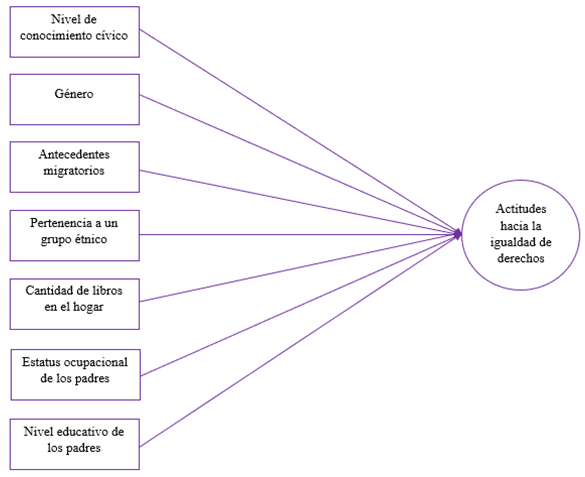
\includegraphics[width=0.8\linewidth,]{images/modelo_1} 

}

\caption{Modelo teórico sobre la relación entre las características del estudiante y sus actitudes hacia la igualdad de derechos}\label{fig:modelo1}
\end{figure}

\hypertarget{investigaciones-centradas-en-el-rol-de-las-escuelas}{%
\subsection{Investigaciones centradas en el rol de las escuelas}\label{investigaciones-centradas-en-el-rol-de-las-escuelas}}

Al plantearse preguntas sobre el rol de las escuelas, diversas investigaciones sobre equidad en educación incorporan en su análisis la teoría del ``efecto de los compañeros''. Según la cual ``{[}\ldots{]} la composición de los alumnos que comparten un aula-escuela afecta los resultados educacionales obtenidos por dichos alumnos y, en consecuencia, que diferentes agrupaciones de estudiantes producirán logros educativos distintos.'' (Bellei, 2013, p.327). Para explicitar de mejor manera la relación entre el efecto de los compañeros y las actitudes hacia la igualdad de derechos, es posible entrecruzar esta perspectiva con una de las corrientes teóricas sobre la discriminación: la teoría del contacto intergrupal (Allport, 1954). Como se explicó anteriormente, esta teoría plantea que, bajo ciertas condiciones, el contacto entre personas de distintos grupos contribuye a reducir la hostilidad intergrupal. Así, se puede hipotetizar que, si se dan dichas condiciones, el contacto con personas de un grupo diferente al propio promovería actitudes positivas con el exogrupo. Este efecto ha sido evaluado en jóvenes europeos el estudio de Isac et al.~(2012), donde se analizó la relación entre la composición del curso en términos de la proporción de estudiantes inmigrantes en el aula y las actitudes hacia la igualdad de derechos para migrantes, concluyendo que existe una asociación positiva entre ambas variables. Asimismo, la investigación de Sincer, Volman, Veen \& Severiens (2020) sobre estudiantes secundarios de Países Bajos concluye que cuando la composición étnica del aula es diversa, los estudiantes poseen más competencias para lidiar con las diferencias.

Como se puede apreciar, los estudios encontrados que analizan la relación entre las actitudes hacia la igualdad de derechos y la composición del aula refieren a jóvenes de países desarrollados y no se han abordado los posibles efectos de la composición de género. Para aportar evidencias sobre esta relación en un país en vías de desarrollo y sobre la composición de género, el presente estudio indagará en el efecto de la composición del aula en términos de la proporción de niñas, de estudiantes de grupos étnicos y de estudiantes migrantes en la escuela. De este modo se buscará comprender si las actitudes hacia la igualdad de derechos varían en función de las características adscriptivas de los estudiantes que componen el aula y, por ende, del contacto con personas del género femenino, pertenecientes a un grupo étnico y/o que han migrado al país. En relación con este punto, se sostendrán tres hipótesis: (1) la proporción de estudiantes en el aula pertenecientes al género femenino posee una asociación positiva con las actitudes hacia la igualdad de derechos, (2) la proporción de estudiantes en el aula pertenecientes a un grupo étnico posee una asociación positiva con las actitudes hacia la igualdad de derechos, y (3) la proporción de estudiantes en el aula que posean antecedentes migratorios tendrá una asociación positiva con las actitudes hacia la igualdad de derechos.

Otro eje de análisis relevante en las investigaciones sobre los procesos de socialización refiere al clima escolar. La investigación de Schulz \& Ainley, 2018 ha evidenciado que las actitudes hacia la igualdad de derechos para grupos étnicos y hacia la igualdad de género se asocian significativamente con el clima escolar. Asimismo, la investigación de Maurissen et al (2020) ha constatado que hay una asociación positiva entre las actitudes hacia la igualdad para migrantes y el clima escolar. Una investigación de una línea de estudios similar a la de la igualdad de derechos ha analizado la asociación entre el clima escolar y la tolerancia a la diversidad en el vecindario utilizando los datos de los países latinoamericanos que participaron en el estudio ICCS 2009, concluyendo que en Chile y Colombia estas variables poseen una relación positiva y significativa, pero con un tamaño efecto bajo (en Chile = 0.09) (Caro \& Schulz, 2012). Sin embargo, existe la posibilidad de que el tamaño de este efecto esté siendo subestimado porque los indicadores que se utilizan para medir el clima escolar son las percepciones de los docentes sobre el clima del aula y los problemas sociales de la escuela. Estos indicadores poseen como problema que la opinión de los docentes podría diferir de la opinión que poseen los estudiantes sobre el clima escolar, siendo poco probable que el grado de tolerancia del estudiante se relacione de forma directa con la percepción del docente sobre el clima escolar. A lo cual se puede añadir que, al tratarse de una encuesta en el marco del espacio laboral, las respuestas de los docentes pueden encontrarse sesgadas por la deseabilidad social. Por ello, en el presente estudio se analizará la relación entre el clima escolar y las actitudes a la igualdad de derechos a partir del set de preguntas sobre el clima en la escuela contestadas por los estudiantes. Al respecto, se sostendrá como hipótesis que en aquellas escuelas en las que los estudiantes perciban un buen clima escolar, se tendrán actitudes más positivas hacia la igualdad de derechos que en otras escuelas.

En una línea de investigación similar, Barber, Torney-Purta y Fennelly (2010), por su parte, y Schulz y Ainley (2018), por otra, han propuesto a partir de sus investigaciones que han propuesto que la apertura a la discusión en el aula genera un ambiente favorable para el desarrollo de actitudes más tolerantes y respetuosas hacia los demás, asociándose positivamente con las actitudes hacia los derechos de los inmigrantes para participar (Barber et al, 2010), las actitudes hacia la igualdad de derechos para grupos étnicos y hacia la igualdad de género (Schulz \& Ainley, 2018). Del mismo modo, otro destacado investigador de los procesos de socialización política, Campbell (2008), plantea que un clima de aula abierta a la discusión permite una comprensión en mayor profundidad de los principios y prácticas democráticas. Asimismo, en el estudio de Caro y Schulz (2012) citado anteriormente, los autores analizaron la relación entre la apertura a la discusión en el aula y la tolerancia a la diversidad en el vecindario, concluyendo que existe una asociación positiva y estadísticamente significativa entre ambas variables en los seis países latinoamericanos que participaron en ICCS 2009 (Chile, Colombia, República Dominicana, Guatemala, México y Paraguay), pero con un tamaño efecto bajo (en Chile = 0.08). Pese a que en una de las investigaciones revisadas se plantea que el tamaño efecto de esta relación es bajo, se ha considerado relevante incluir la percepción de los estudiantes sobre la apertura a la discusión en el aula en esta investigación debido a que este efecto ha sido analizado en otros estudios y, en ese estudio en particular, el efecto podría estar subestimado porque se no se utilizaron las respuestas de los estudiantes sobre la apertura a la discusión en el aula, sino que las respuestas de los docentes. En relación con este punto, se sostendrá como hipótesis que en aquellas escuelas en las que los estudiantes perciban un clima más abierto a la discusión en el aula, se tendrán actitudes más positivas hacia la igualdad de derechos que en otras escuelas.

En suma, a partir los antecedentes revisados sobre la asociación entre las características de la escuela y las actitudes hacia la igualdad de derechos, se propone el siguiente modelo teórico:

\begin{figure}[!ht]

{\centering 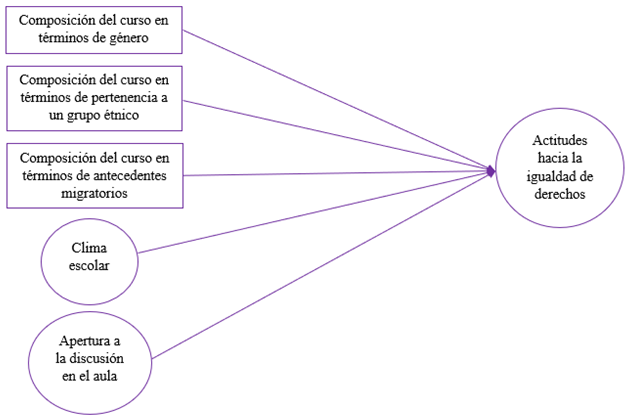
\includegraphics[width=0.8\linewidth,]{images/modelo_2} 

}

\caption{Modelo teórico sobre la relación entre las características de la escuela y las actitudes hacia la igualdad de derechos}\label{fig:modelo2}
\end{figure}

Por último, como se ha explicado en la introducción, el interés principal de este proyecto de investigación es evaluar si la relación entre las características del estudiante y sus actitudes hacia la igualdad de derechos se puede moderar por alguna/s de las características de la escuela destacadas frecuentemente en las investigaciones previas. Así, se espera aportar a la comprensión de cuáles prácticas y características de las escuelas permiten disminuir las diferencias individuales en las actitudes hacia la igualdad de derechos. Por lo tanto, la hipótesis principal de este estudio es de carácter exploratorio, aunque se sostiene en las múltiples evidencias previas sobre los efectos directos de la composición del aula, la apertura a la discusión y el clima escolar en las actitudes positivas hacia la igualdad de derechos (Isac et al, 2012; Sincer et al, 2020; Barber et al, 2010; Schulz \& Ainley, 2018; Caro \& Schulz, 2012; Maurissen et al, 2020). Además, se tiene como antecedente que el estudio de Isac et al (2012) ha evidenciado que en aquellos países donde la composición del aula en términos de proporción de estudiantes migrantes es más diversa, los estudiantes nativos poseen actitudes más positivas hacia la igualdad de derechos que en el resto de los países. Sin embargo, no se poseen evidencias sobre la interacción entre las características de los estudiantes y las características de la escuela.

Se sostiene como hipótesis que alguna/s de las características de las escuelas (destacadas frecuentemente en investigaciones previas) permitirá moderar el efecto que tienen las características individuales sobre las actitudes hacia la igualdad de derechos. En otras palabras, se espera que alguna de estas características disminuya las diferencias individuales en las actitudes hacia la igualdad de derechos. Para ello, se evaluará el modelo teórico que se presenta a continuación.

\begin{figure}[!ht]

{\centering 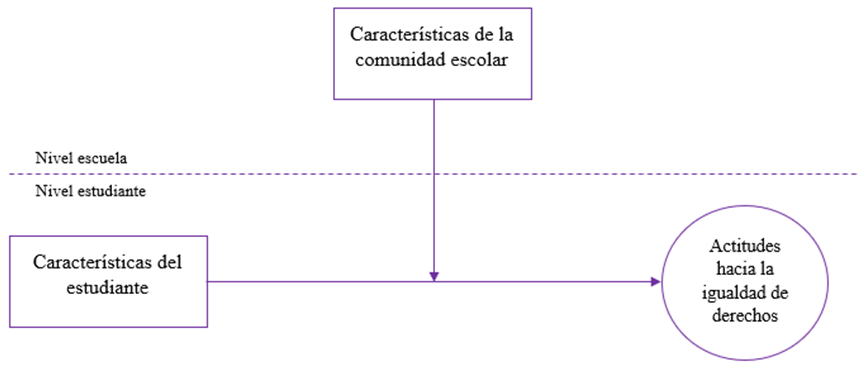
\includegraphics[width=0.8\linewidth,]{images/modelo_3} 

}

\caption{Modelo teórico sobre la relación entre las características del estudiante y sus actitudes hacia la igualdad de derechos, moderada por las características de la escuela}\label{fig:modelo3}
\end{figure}

\hypertarget{especificaciones-metodoluxf3gicas}{%
\chapter{Especificaciones metodológicas}\label{especificaciones-metodoluxf3gicas}}

\hypertarget{datos}{%
\section{Datos}\label{datos}}

Esta investigación utilizará los datos del último estudio Internacional sobre Educación Cívica y Ciudadana (ICCS) de la IEA, el cual consiste en una evaluación estandarizada que permite evaluar cómo las escuelas preparan a sus estudiantes para asumir su rol de ciudadanos, proporcionando evidencia sobre la orientación moral a los Derechos Humanos y la justicia social, el conocimiento cívico y las percepciones sobre el clima escolar de estudiantes de distintas partes del mundo (Schulz, Ainley, Cox et al, 2016). La encuesta fue realizada a una muestra representativa de los estudiantes matriculados en octavo grado en 24 países, siempre que la edad promedio de ese nivel fuera 13,5 años o más (de lo contrario, se define el noveno grado como la población objetivo) (IEA, s.f.). En Chile este estudio incorporó a 5.081 estudiantes de 8°básico de 178 escuelas, entre los cuales el 49,3\% se identificó con el género femenino y el 50,7\% con el género masculino. La muestra incluye establecimientos de todas las regiones, dependencias administrativas y zonas geográficas del país (Agencia de Calidad de la Educación, s.f.). Cabe destacar que se muestreo sólo una clase por escuela, por lo que los datos corresponden a estudiantes que no sólo pertenecen a la misma escuela, sino que comparten en el aula de clases (Schulz, Carstens, Losito, \& Fraillon, 2018).

\hypertarget{variables}{%
\section{Variables}\label{variables}}

En esta sección se presentarán las variables a utilizar y sus respectivos códigos en la base de datos ICCS.

\hypertarget{indicadores-de-las-actitudes-hacia-la-igualdad-de-derechos}{%
\subsection{Indicadores de las actitudes hacia la igualdad de derechos}\label{indicadores-de-las-actitudes-hacia-la-igualdad-de-derechos}}

En la encuesta se realiza una serie de preguntas referidas a las actitudes hacia la igualdad de derechos: de género, para grupos étnicos o raciales, y para homosexuales. Este set de preguntas se establece como el objeto central de este estudio. Estas actitudes son medidas en función del grado de acuerdo con diferentes afirmaciones en una escala de 1 a 4, donde: 1. Muy de acuerdo, 2. De acuerdo, 3. En desacuerdo, 4. Muy en desacuerdo. Para facilitar el análisis, las categorías de respuesta serán recodificadas de modo que 1 represente ``Muy en desacuerdo'', 2 ``En desacuerdo'', 3 ``De acuerdo'' y 4 ``Muy de acuerdo''.

Como se enuncio anteriormente, para medir las actitudes hacia la igualdad de género y hacia la igualdad de derechos para grupos étnicos se seguirá el modelo de medida propuesto en el artículo de Miranda y Castillo (2018). Por lo tanto, sólo se incorporarán los indicadores que refieren específicamente a la igualdad de derechos, pese a que las escalas originales incorporan otros indicadores. Como en dicho artículo no se incorpora un análisis de la escala de actitudes hacia la igualdad de derechos para homosexuales (debido a que es una escala que no estaba en el estudio ICCS 2009), se ha seguido el mismo criterio utilizado por los autores de dicho artículo para definir si excluir o no alguno de los indicadores. En este sentido, se ha decidido no excluir ninguno de los indicadores de dicha escala debido a que se ha considerado que todos refieren específicamente a la igualdad de derechos y no a otros constructos. Se estimará el ajuste de las variables dependientes en un modelo donde se diferenciarán las tres variables latentes (una por cada grupo) y se explicitará que las tres variables latentes están correlacionadas entre sí.

Los indicadores y sus códigos se presentan a continuación:

\begin{itemize}
\item
  Existen diferentes puntos de vista sobre los roles de mujeres y hombres en la sociedad. ¿Cuán de acuerdo o en desacuerdo estás tú con las siguientes declaraciones?

  \begin{itemize}
  \tightlist
  \item
    Los hombres y las mujeres deberían tener las mismas oportunidades de participar en el gobierno. (IS3G24A)
  \item
    Los hombres y las mujeres deberían tener los mismos derechos en todos los aspectos. (IS3G24B)
  \item
    Los hombres y las mujeres deberían recibir el mismo pago cuando están haciendo los mismos los trabajos. (IS3G24E)
  \end{itemize}
\item
  Existen diferentes puntos de vista sobre los derechos y responsabilidades de los diferentes en la sociedad. ¿Cuán de acuerdo o en desacuerdo estás tú con las siguientes declaraciones?

  \begin{itemize}
  \tightlist
  \item
    En Chile todos los grupos étnicos y raciales deberían tener la misma oportunidad de acceder a una buena educación. (IS3G25A)
  \item
    En Chile todos los grupos étnicos y raciales deberían tener la misma oportunidad de conseguir buenos trabajos. (IS3G25B)
  \item
    Las escuelas deberían enseñar a los estudiantes a respetar a los miembros de todos los grupos étnicos y raciales. (IS3G25C)
  \item
    Los miembros de todos los grupos étnicos y raciales deberían tener los mismos derechos y responsabilidades. (IS3G25E)
  \end{itemize}
\item
  ¿En qué medida estás de acuerdo o en desacuerdo con las siguientes afirmaciones respecto a la homosexualidad?

  \begin{itemize}
  \tightlist
  \item
    Las personas del mismo sexo deberían tener derecho a casarse entre sí. (LS3G08A)
  \item
    Dos personas del mismo sexo deberían tener el derecho de adoptar hijos. (LS3G08B)
  \item
    Los homosexuales deberían tener los mismos derechos que los demás ciudadanos. (LS3G08C)
  \item
    Todos los colegios deberían aceptar a homosexuales. (LS3G08D)
  \item
    Los homosexuales deberían tener el derecho de postularse para cualquier cargo político o público. (LS3G08E)
  \end{itemize}
\end{itemize}

\hypertarget{indicadores-de-las-variables-independientes}{%
\subsection{Indicadores de las variables independientes}\label{indicadores-de-las-variables-independientes}}

\hypertarget{nivel-estudiante}{%
\subsubsection{Nivel estudiante}\label{nivel-estudiante}}

\textbf{Nivel de conocimiento cívico (PV1CIV)}

\begin{itemize}
\tightlist
\item
  La variable corresponde al puntaje asignado al nivel de conocimiento cívico del estudiante, como resultado de un procedimiento basado en la teoría de respuesta al ítem para estimar los valores plausibles de conocimiento cívico del estudiante en base a su respuesta a 87 preguntas. Los valores de esta variable varían entre el 0 y el 800, donde un puntaje mayor indica un mayor nivel de conocimiento cívico.
\end{itemize}

\textbf{Sexo (S\_Gender)}

\begin{itemize}
\tightlist
\item
  Esta variable distingue entre hombre (0) y mujer (1).
\end{itemize}

\textbf{Antecedentes migratorios (IS3G04A)}

\begin{itemize}
\tightlist
\item
  Al estudiante se le pregunta en qué país nació (IS3G04A) y en qué países nacieron sus padres (país en qué nació la madre = IS3G04B; país en qué nació el padre = IS3G04C). Haber nacido en Chile fue codificado como 1, y haber nacido en cualquier otro país fue codificado como 0.
\end{itemize}

\textbf{Pertenencia a un grupo étnico (IS3G02BN)}

\begin{itemize}
\tightlist
\item
  Al estudiante se le solicita que escriba las tres palabras que mejor lo describen. Si entre estas palabras el estudiante escribe un pueblo nativo chileno, su respuesta es codificada como ``15202''.
\end{itemize}

\textbf{Nivel socioeconómico de la familia}

En la encuesta existen tres variables referidas al nivel socioeconómico de la familia del estudiante. Como se mencionó anteriormente, se evaluará el efecto de cada variable por separado. Las preguntas y sus categorías de respuesta se presentan a continuación:

\begin{itemize}
\item
  \textbf{\emph{El nivel educativo alcanzado más alto entre los dos padres (S\_HISCED).}} Para construir esta variable al estudiante se le presentan dos preguntas: 1) ¿Cuál es el nivel más alto de educación completado por su madre o tutora?, 2) ¿Cuál es el nivel más alto de educación completado por su padre o tutor? Ambas preguntas tienen las mismas opciones de respuesta: 1) Una carrera universitaria o estudios de posgrado (magister o doctorado), 2) Una carrera profesional o técnica, 3) Enseñanza media, 4) Enseñanza básica, 5) No completo la enseñanza básica. Se compararon las respuestas de los estudiantes a estas dos preguntas y se construyó una nueva variable (S\_HISCED), cuyo valor corresponde al nivel educativo más alto completado por uno de los dos padres (o tutores).
\item
  \textbf{\emph{La ocupación de mayor estatus entre los dos padres (S\_HISEI).}} Para construir esta variable se le presentan cuatro preguntas abiertas al estudiante: 1) ¿Cuál es el trabajo principal de su madre o tutora? (por ejemplo, maestro de escuela secundaria, ayudante de cocina, gerente de ventas), 2) ¿Qué hace tu madre o tutora en su trabajo principal? (por ejemplo, enseña a los estudiantes de secundaria, ayuda al cocinero a preparar las comidas en un restaurante, gestiona un equipo de ventas), 3) ¿Cuál es el trabajo principal de su padre o tutor? (por ejemplo, maestro de escuela secundaria, ayudante de cocina, gerente de ventas), 4) ¿Qué hace tu padre o tutor masculino en su trabajo principal? (por ejemplo, enseña a los estudiantes de secundaria, ayuda al cocinero a preparar las comidas en un restaurante, gestiona un equipo de ventas). El valor asignado a las respuestas de estas preguntas se determina en función de las puntuaciones en el esquema de clasificación ocupacional ISCO-08 y se recodifican a puntuaciones SEI (índice socioeconómico de Duncan). Después de esta recodificación, se compara el puntaje del estatus ocupacional de la madre (o tutora) con el puntaje del estatus ocupacional del padre (o tutor) para crear una nueva variable, cuyo valor corresponde al puntaje del estatus ocupacional más alto entre los dos padres (o tutores). Esta variable será la que se incorporará en el análisis (S\_HISEI).
\item
  \textbf{\emph{La cantidad de libros en el hogar (IS3G11).}} Al estudiante se le pregunta ``¿Aproximadamente cuántos libros hay en tu casa? No cuente revistas, periódicos, historietas, libros electrónicos o sus libros escolares'' y se le presentan 5 categorías de respuesta: 1) Ninguno o muy pocos (0-10 libros), 2) Suficiente para llenar un estante (11-25 libros), 3) Suficiente para llenar dos estantes (26-100 libros), 4) Suficiente para llenar dos estanterías (101-200 libros) y 5) Suficiente para llenar tres o más estanterías (más de 200 libros).
\end{itemize}

\hypertarget{nivel-escuela}{%
\subsubsection{Nivel escuela}\label{nivel-escuela}}

\textbf{Composición del curso en términos de género}

Se creará una variable que representará la proporción de mujeres en el curso.

\textbf{Composición del curso en términos de antecedentes migratorios}

Se creará una variable que representará la proporción de estudiantes con antecedentes migrantes en el curso.

\textbf{Composición del curso en términos de la proporción de estudiantes pertenecientes a un grupo étnico}

Se creará una variable que representará la proporción de estudiantes pertenecientes a un grupo étnico en el curso.

\textbf{Apertura a la discusión en el aula}

Siguiendo las sugerencias expuestas en el estudio de Campbell (2008), se ha decidido promediar por escuela las respuestas de los estudiantes a cada uno de los indicadores de la escala con el objetivo de obtener una medida que represente de mejor manera la apertura a la discusión en el aula\footnote{Antes de incorporar esta variable de control en el modelo, se centrará la variable al promedio del colegio con el objetivo de despejar el efecto individual del efecto de la escuela.}, debido a que las percepciones de cada uno de los estudiantes pueden estar influidas por otros factores (como el compromiso político del joven). De modo que todos los estudiantes pertenecientes a una misma aula recibirán la misma puntuación en cada uno de los indicadores. La variable latente se estimará basándose en los indicadores promediados por aula. Sin embargo, para realizar una estimación precisa del efecto del colegio, se incluirá como variable de control la percepción de cada estudiante sobre la apertura a la discusión en el aula para despejar la posibilidad de que los efectos se deban a la percepción individual de cada estudiante. Esta variable de control también se incorporará al modelo como variable latente, pero como una variable de nivel individual.

En relación con los indicadores de la escala, cabe destacar que al estudiante se le pregunta la frecuencia en qué ocurren determinadas situaciones durante las clases, pidiéndole que escoja entre los siguientes grados de frecuencia: 1) Nunca, 2) Raramente, 3) A veces, 4) A menudo. A continuación se expone la pregunta general y los distintos indicadores, con sus respectivos códigos.

\begin{itemize}
\item
  Cuando se discuten temas políticos o sociales durante las clases regulares, ¿con qué frecuencia suceden las siguientes cosas?

  \begin{itemize}
  \tightlist
  \item
    Los maestros alientan a los estudiantes a tomar sus propias decisiones. (IS3G17A)
  \item
    Los maestros alientan a los estudiantes a expresar sus opiniones. (IS3G17B)
  \item
    Los estudiantes presentan eventos políticos actuales para su discusión en clase. (IS3G17C)
  \item
    Los estudiantes expresan opiniones en clase incluso cuando sus opiniones son diferentes de la mayoría de los otros estudiantes. (IS3G17D)
  \item
    Los maestros alientan a los estudiantes a discutir los problemas con personas que tienen opiniones diferentes. (IS3G17E)
  \item
    Los maestros presentan varios lados de los problemas cuando los explican en clase. (IS3G17F)
  \end{itemize}
\end{itemize}

\textbf{Clima escolar}

En consideración de los argumentos expuestos en la justificación de cómo se medirá la variable apertura a la discusión en el aula, se ha decidido medir el clima escolar siguiendo la misma lógica. En otras palabras, debido a que la percepción del clima escolar de cada estudiante puede estar influida por características individuales y, por ende, puede no representar a cabalidad cómo es el clima escolar de ese colegio, se ha decidido estimar un promedio por escuela de cada uno de los indicadores de la variable clima escolar. Así, la variable latente a estimar se basará en indicadores que tienen la misma puntuación para todos los estudiantes de una misma escuela. Asimismo, tal cómo se hará con la variable anterior, se incorporará como variable de control las percepciones individuales sobre el clima en el aula, para lo cual se centrarán los indicadores al promedio de la escuela antes de estimar la variable latente.

Respecto a los indicadores del clima escolar, cabe mencionar que en el cuestionario ICCS 2016 se realizan dos series de preguntas sobre el clima escolar, una referida a la percepción del estudiante acerca de las relaciones interpersonales en la escuela (tanto entre los profesores y los estudiantes, como entre los estudiantes) y otra enfocada en la vivencia de situaciones de violencia física, emocional y/o verbal en la escuela. A continuación se presentan los indicadores:

\textbf{\emph{Relaciones interpersonales en la escuela}}

Al estudiante se le pregunta su grado de acuerdo con diversas frases relacionadas con las interacciones tanto entre los profesores y los estudiantes, como entre estudiantes. Se le ofrecen cuatro alternativas de respuesta: 1) Muy de acuerdo, 2) De acuerdo, 3) En desacuerdo, 4) Totalmente en desacuerdo. Con el objetivo de facilitar el análisis, estas categorías de respuesta serán recodificadas, de modo que 1 represente ``Totalmente en desacuerdo'', 2 ``En desacuerdo, 3 ``De acuerdo'', 4 ``Muy de acuerdo''.

\begin{itemize}
\item
  ¿Cuán de acuerdo o en desacuerdo estás con las siguientes declaraciones sobre los maestros y estudiantes de tu escuela?

  \begin{itemize}
  \tightlist
  \item
    La mayoría de mis maestros me tratan con justicia. (IS3G19A)
  \item
    Los estudiantes se llevan bien con la mayoría de los maestros. (IS3G19B)
  \item
    La mayoría de los maestros están interesados en el bienestar de los estudiantes. (IS3G19C)
  \item
    La mayoría de mis maestros escuchan lo que tengo que decir. (IS3G19D)
  \item
    Si necesito ayuda adicional, la recibo de mis maestros. (IS3G19E)
  \item
    La mayoría de los maestros evitarían que los estudiantes sean intimidados. (IS3G19F)
  \item
    La mayoría de los estudiantes de mi escuela se tratan con respeto. (IS3G19G)
  \item
    La mayoría de los estudiantes de mi escuela se llevan bien entre ellos. (IS3G19H)
  \item
    Mi escuela es un lugar donde los estudiantes se sienten seguros. (IS3G19I)
  \end{itemize}
\end{itemize}

\textbf{\emph{Situaciones de violencia física, emocional o verbal}}
Al estudiante se le pregunta con qué frecuencia han ocurrido en la escuela determinadas situaciones relacionadas a violencia escolar, pidiéndole que escoja entre los siguientes grados de frecuencia: 1) Nunca, 2) Menos de una vez al mes, 3) 1 a 5 veces al mes, 4) más de 5 veces al mes. A continuación se presenta la pregunta general y los indicadores.

\begin{itemize}
\item
  El Bullying se define como la actividad de comportamiento repetido y agresivo destinado a lastimar a alguien ya sea física, emocional, verbal o a través de la comunicación por internet. Durante el año escolar actual, ¿con qué frecuencia sucedió alguna de las siguientes situaciones en este colegio?

  \begin{itemize}
  \tightlist
  \item
    Un estudiante ha reportado al director de la escuela comportamientos agresivos o destructivos de otros estudiantes. (IC3G06A)
  \item
    Un estudiante informó al director de la escuela que él / ella era por un profesor. (IC3G06B)
  \item
    Un maestro informó al director de la escuela que un estudiante era por otros estudiantes. (IC3G06C)
  \item
    Un maestro informó al director de la escuela que un alumno ayudó a otro estudiante al que le estaban haciendo bullying. (IC3G06D)
  \item
    Un maestro informó al director de la escuela que él / ella estaba siendo por estudiantes. (IC3G06E)
  \item
    Un padre informó al director de la escuela que su hijo / hija fue por otros estudiantes. (IC3G06F)
  \end{itemize}
\end{itemize}

\hypertarget{muxe9todos}{%
\section{Métodos}\label{muxe9todos}}

Para responder a los objetivos de este proyecto de investigación se ha decidido utilizar una estrategia de investigación cuantitativa, principalmente por dos motivos. Por un lado, debido a que actualmente existen datos secundarios disponibles que abordan toda la información que requiero analizar, en la población de interés (jóvenes en edad escolar). Estos datos se encuentran disponibles en el estudio ICCS 2016, una prueba estandarizada a nivel internacional que fue construida por un equipo de investigadores expertos en la temática de educación cívica. Cabe destacar que este estudio posee como precedente dos estudios anteriores (CIVED 1999 y ICCS 2009), por lo que la construcción de este tercer estudio se ha servido de la experiencia recopilada en las investigaciones anteriores y se han realizado las mejoras que se consideraron necesarias. En consecuencia, se puede afirmar que son datos de buena calidad. Por otro lado, he considerado que la estrategia cuantitativa es la más adecuada para responder al objetivo general de este estudio debido a que a través de técnicas estadísticas como las regresiones es posible estimar efectos de interacción entre las variables. La estimación de efectos de interacción entre variables me permite evaluar con precisión si alguna/s de la/s característica/s de la escuela que se incorporan en el análisis posee/n la capacidad de moderar la relación existente entre las características adscritas del estudiante y sus actitudes hacia la igualdad de derechos.

El plan de análisis de este proyecto de investigación consta de dos partes, uno enfocado en evaluar los modelos de medida de las variables latentes y otro enfocado en testear las hipótesis.

En primer lugar, se estimará un análisis factorial confirmatorio multinivel con el objetivo de evaluar si la dimensionalidad propuesta para medir las actitudes hacia la igualdad de derechos presenta un ajuste adecuado (la propuesta se presenta con mayor detalle en el acápite ``Variables''). Además, se estimará un análisis factorial confirmatorio multinivel para las variables independientes que son variables latentes (clima escolar y apertura a la discusión en el aula). Se utilizarán los criterios de evaluación de la bondad del ajuste del modelo propuestos por Brown (2008): (1) Chi-square mayor que 0.05; (2) Chi-square ratio menor que 3; (3) CFI mayor que 0.95; (4) TLI mayor que 0.95; y (5) RMSEA menor que 0.08.

En segundo lugar, se tienen dos opciones para testear las hipótesis, pero no es posible definir en este momento cuál de las dos opciones se implementará. Aunque cabe destacar que, sin lugar a duda, el modelamiento será multinivel. Esta decisión se fundamenta en que, como las encuestas se realizan a más de un estudiante de cada escuela, no es posible suponer la existencia de independencia entre los casos\footnote{Antes de incorporar esta variable de control en el modelo, se centrará la variable al promedio del colegio con el objetivo de despejar el efecto individual del efecto de la escuela.}, siendo lo más apropiado que el análisis se realice agrupando a los estudiantes por escuela.

Se han formulado dos opciones debido a que se desea privilegiar ante todo realizar un análisis que sea transparente y reproducible, para lo cual se utilizará el software libre R. La primera opción es estimar modelos de ecuaciones estructurales multinivel debido a que la variable dependiente en este estudio no es una variable observada, sino que es una variable latente (es decir, fue medida a partir de varios indicadores) y esta técnica estadística está específicamente diseñada para el análisis de variables latentes. En esta línea, un estudio de simulación Monte Carlo (Rdz-Navarro \& Asún, 2016) establece que, al trabajar con variables latentes, emplear esta forma de estimación estadística permite reducir el error de medida, en comparación a utilizar otras técnicas que buscan dar cuenta de una puntuación observada (ya sea a partir de un índice sumatorio, puntuaciones factoriales o estimaciones derivadas de la teoría de respuesta al ítem). Por lo tanto, en el caso de que se desarrolle una actualización de la librería ``lavaan'' (la cual permite estimar modelos de ecuaciones estructurales multinivel en R) donde se incorpore la posibilidad de estimar SEM de dos niveles con pendientes aleatorias, se estimarán modelos de ecuaciones estructurales multinivel para testear las hipótesis. Sin embargo, el creador de ``lavaan'' señala que, pese a ser parte de sus planes futuros para el desarrollo de la librería, no le es posible estimar cuánto tiempo tardará en implementar esta función. Por este motivo es que he formulado otra opción para el testeo de las hipótesis, en caso de que no se implemente la función en el corto plazo. La segunda opción consiste en la estimación de puntuaciones factoriales para testear las hipótesis con modelos de regresiones multinivel a través de la librería ``lme4''. Cabe destacar que esta segunda opción generaría que, probablemente, los resultados del estudio tengan más error de medida (en comparación a usar una técnica especialmente diseñada para el análisis de variables latentes).

Con el objetivo de asumir un compromiso con el desarrollo de una ciencia social abierta, se subirá un pre-registro de las hipótesis a la plataforma Open Science Framework (OSF) y se creará un repositorio en la plataforma GitHub para ir subiendo los códigos de análisis estadístico con sus respectivos resultados.

\hypertarget{anuxe1lisis-factorial-confirmatorio-variables-dependientes}{%
\chapter{Análisis factorial confirmatorio: Variables dependientes}\label{anuxe1lisis-factorial-confirmatorio-variables-dependientes}}

\begin{Shaded}
\begin{Highlighting}[]
\NormalTok{data_tt =}\StringTok{ }\NormalTok{data1 }\OperatorTok\StringTok{ }\KeywordTok{select}\NormalTok{(IS3G24A,IS3G24B,IS3G24E,IS3G25A,IS3G25B,IS3G25C,IS3G25E,LS3G08A,LS3G08B,LS3G08C,LS3G08D,LS3G08E,idschool) }\OperatorTok\StringTok{ }\KeywordTok{as.data.frame}\NormalTok{()}
\NormalTok{model_tt <-}\StringTok{ '}
\StringTok{f.genero =~ IS3G24A + IS3G24B + IS3G24E }

\StringTok{f.etnico =~ IS3G25A + IS3G25B + IS3G25C + IS3G25E}

\StringTok{f.homosexual =~ LS3G08A + LS3G08B + LS3G08C + LS3G08D + LS3G08E}

\StringTok{f.genero ~~ f.etnico }
\StringTok{f.genero ~~ f.homosexual}
\StringTok{f.etnico ~~ f.homosexual'}

\NormalTok{fit_tt<-}\StringTok{ }\KeywordTok{cfa}\NormalTok{(model_tt, }\DataTypeTok{data=}\NormalTok{data_tt, }\DataTypeTok{ordered=}\KeywordTok{c}\NormalTok{(}\StringTok{"IS3G24A"}\NormalTok{,}\StringTok{"IS3G24B"}\NormalTok{,}\StringTok{"IS3G24E"}\NormalTok{,}\StringTok{"IS3G25A"}\NormalTok{,}\StringTok{"IS3G25B"}\NormalTok{,}\StringTok{"IS3G25C"}\NormalTok{,}\StringTok{"IS3G25E"}\NormalTok{,}\StringTok{"LS3G08A"}\NormalTok{,}\StringTok{"LS3G08B"}\NormalTok{,}\StringTok{"LS3G08C"}\NormalTok{,}\StringTok{"LS3G08D"}\NormalTok{,}\StringTok{"LS3G08E"}\NormalTok{), }\DataTypeTok{cluster =} \StringTok{'idschool'}\NormalTok{)}
\KeywordTok{summary}\NormalTok{(fit_tt, }\DataTypeTok{fit.measures=}\NormalTok{T, }\DataTypeTok{standardized=}\NormalTok{T)}
\end{Highlighting}
\end{Shaded}

\textbf{Indicadores de ajuste del modelo}

\begin{longtable}[]{@{}lll@{}}
\toprule
& Standard & Robust\tabularnewline
\midrule
\endhead
Chi-square (P-value) & 878,808 (0,000) & 1659,773 (0,000)\tabularnewline
Chi-square Ratio (df) & 17,231 (51) & 32,544 (51)\tabularnewline
CFI & 0,998 & 0,991\tabularnewline
TLI & 0,998 & 0,988\tabularnewline
RMSEA (P-value) & 0,057 (0,000) & 0,079 (0,000)\tabularnewline
\bottomrule
\end{longtable}

Siguiendo los criterios de bondad de ajuste propuestos por Brown (2008), es posible afirmar que según los indicadores relativos al Chi-square el modelo de medida no presentaría un ajuste adecuado. Sin embargo, esta prueba suele verse afectada cuando se trabaja con tamaños muestrales grandes, por lo que se deben analizar también los otros tres indicadores de ajuste del modo. Los otros tres indicadores se encuentran dentro de los criterios establecidos por Brown, generando evidencias de un nivel de ajuste adecuado. Por consiguiente, se ha decidido utilizar este modelo de medida para las variables dependientes debido a que presenta un ajuste parcialmente adecuado.

\hypertarget{bibliografuxeda}{%
\chapter*{Bibliografía}\label{bibliografuxeda}}
\addcontentsline{toc}{chapter}{Bibliografía}

Abramo, L. (2017). CEPAL: Pese a avances recientes, América Latina sigue siendo la región más desigual del mundo. Revisado el 8 de mayo, 2020, en: \url{https://www.cepal.org/es/comunicados/cepal-pese-avances-recientes-america-latina-sigue-siendo-la-region-mas-desigual-mundo}

Agencia de Calidad de la Educación. (s.f.). ICCS: Estudio Internacional de Educación Cívica y Formación Ciudadana. Revisado el 30 de julio, 2020, en: \url{https://www.agenciaeducacion.cl/estudios/estudios-internacionales/iccs/}

Allport, G. (1954). The nature of prejudice. Reading, MA: Perseus Book Publishing.

Araujo, K. (2013). La Igualdad en el Lazo Social: Procesos Sociohistóricos y Nuevas Percepciones de la Desigualdad en la Sociedad Chilena. Dados - Revista de Ciências Sociais, 56(1), 109-132.

Barber, C., Torney-Purta, J. y Fennelly, K. (2010). Adolescents' Attitudes toward Immigrants' Rights and Nationalism in 25 Countries. Conference: 4th IEA International Research Conference (IRC-2010). At: Gothenburg, Sweden.

Bárcena, A., Prado, A., Abramo, L. \& Pérez, R. (2016). La matriz de la desigualdad social en América Latina. Naciones Unidas, Comisión Económica para América Latina y el Caribe (CEPAL): Santiago.

Bellei, C. (2013). El estudio de la segregación socioeconómica y académica de la educación chilena. Estudios pedagógicos (Valdivia), 39(1), 325-345.

Beltrán, M. (2004). Tolerancia y Derechos Humanos. Política y cultura, (21), 179-189. Revisado el 18 de julio, 2020, en: \url{http://www.scielo.org.mx/scielo.php?script=sci_arttext\&pid=S0188-77422004000100012\&lng=es\&tlng=es}.

Brown, T. (2008). Confirmatory Factor Analysis for Applied Research. Second edition. New York: The Guilford Press.
Burchardt, H. (2008). Desigualdad y democracia. Nueva Sociedad (215), pp.~79-94.

Campbell, D. (2008). Voice in the Classroom: How an Open Classroom Climate Fosters Political Engagement Among Adolescents. Political Behavior, 30(4), 437--454. \url{https://doi.org/10.1007/s11109-008-9063-z}

Caro, D. H., \& Schulz, W. (2012). Ten Hypotheses about Tolerance toward Minorities among Latin American Adolescents. Citizenship, Social and Economics Education, 11(3), 213-234. \url{https://doi.org/10.2304/csee.2012.11.3.213}

Conde, F. (2014). Desigualdad, discriminación y pedagogía de la igualdad. Revista Actividades Investigativas en Educación, Universidad de Costa Rica, (14), pp.1-20.

Comisión Económica para América Latina y el Caribe (CEPAL). (2017). Panorama Social de América Latina, 2016. Naciones Unidas: Santiago. Revisado el 8 de mayo, 2020, en: \url{https://repositorio.cepal.org/bitstream/handle/11362/41598/4/S1700567_es.pdf}

De Groof, S., Elchardus, M., Franck E. \& Kavadias, D. (2008). The Influence of Civic Knowledge versus Democratic School Experiences on Ethnic Tolerance of Adolescents. A Multilevel analysis. Paper presented at the 3rd IEA International Research Conference, September 18-20, 2008, Taipei: Onderzoeksgroep TOR, Vakgroep Sociologie, Vrije Universiteit Brussel - TOR 2008/31.

Durkheim, E. (2000). Educación y sociología. Barcelona: Península. (original publicado en 1922).

Duckitt, J. (1992). Psychology and prejudice. A Historical Analysis and Integrative Framework. American Psychological Association, 47(10), 1182-1193.

Garretón, M. A. (2015). Nueva problemática sociohistórica e igualdad. En Garretón, M.A.~(Ed.) Las ciencias sociales en la trama de Chile y América Latina. Santiago, Chile: LOM.

Gorodzeisky, A. \& Semyonov, M. (2009) Terms of exclusion: public views towards admission and allocation of rights to immigrants in European countries, Ethnic and Racial Studies, 32(3), 401-423. \url{https://doi.org/10.1080/01419870802245851}

Honneth, A. (2010). Reconocimiento y menosprecio. Sobre la fundamentación normativa de una teoría social. Buenos Aires, Argentina: Katz.

Huddleston, T., \& Vink, M.P. (2015). Full membership or equal rights? The link between naturalisation and integration policies for immigrants in 29 European states. Comparative Migration Studies, 3(1). DOI: 10.1186/s40878-015-0006-7

IEA. (s.f.). ICCS. International Civic and Citizenship Education Study. Revisado el 30 de julio, 2020, en: \url{https://www.iea.nl/studies/iea/iccs}

Isac, M. M., Maslowski, R., \& Van der Werf, G. (2012). Native student attitudes towards equal rights for immigrants. A study in 18 European countries. Journal of Social Science Education, 11(1), 7-26. \url{https://doi.org/10.2390/jsse-v11-i1-1189}

Madeira, AF., Costa-Lopes, R., Dovidio, JF., Freitas, G. \& Mascarenhas, MF. (2019). Primes and Consequences: A Systematic Review of Meritocracy in Intergroup Relations. Frente. Psychol, 10. \url{https://doi.org/10.3389/fpsyg.2019.02007}

Ministerio de Educación (Mineduc). (2016a). Orientaciones curriculares para el desarrollo del plan de Formación Ciudadana. Santiago, Chile: Maval.

Ministerio de Educación (Mineduc). (2016b). Orientaciones para la elaboración del plan de Formación Ciudadana. Revisado el 20 de junio, 2020, en: \url{https://formacionciudadana.mineduc.cl/wp-content/uploads/sites/46/2016/04/DEG-OrientacionesPFC-intervenible-AReader_FINAL.pdf}

Ministerio de Educación (Mineduc). (2017). Orientaciones para la apropiación de las bases curriculares de 7° básico a 2° medio. Revisado el 22 de junio, 2020, en: \url{https://media.mineduc.cl/wp-content/uploads/sites/28/2017/05/Orientaciones-apropiacion-BC-7\%C2\%BA-2\%C2\%BAM-web-corregido.pdf}

Miranda, D. \& Castillo, J. (2018). Measurement Model and Invariance Testing of Scales Measuring Egalitarian Values in ICCS 2009. En Sandoval-Hernández, A., Isac, M., \& Miranda, D. (Eds.). Teaching Tolerance in a Globalized World (pp.~19-32). International Association for the Evaluation of Educational Achievement (IEA).

Miranda, D., Castillo, J., \& Cumsille, P. (2018). The Political Socialization of Attitudes Toward Equal Rights from a Comparative Perspective. En Sandoval-Hernández, A., Isac, M., \& Miranda, D. (Eds.). Teaching Tolerance in a Globalized World (pp.~103-124). International Association for the Evaluation of Educational Achievement (IEA).

Organización de las Naciones Unidas (ONU). (2011). Declaración de las Naciones Unidas sobre educación y formación en materia de Derechos Humanos. Revisado el 14 de mayo, 2020, en: \url{http://www.derechoshumanos.unlp.edu.ar/assets/files/documentos/declaracion-de-naciones-unidas-sobre-educacion-y-formacion-en-materia-de-derechos-humanos.pdf}

Organización de las Naciones Unidas (ONU). (s.f.). LA DECLARACIÓN UNIVERSAL DE DERECHOS HUMANOS: FUNDAMENTO DE LAS NORMAS INTERNACIONALES DE DERECHOS HUMANOS. Revisado el 14 de agosto, 2020, en: \url{https://www.un.org/es/documents/udhr/law.shtml}

Organización de las Naciones Unidas (ONU). (2018). La tolerancia, ni indulgencia ni indiferencia: respeto. Revisado el 20 de septiembre, 2019, en: \url{https://www.un.org/es/events/toleranceday/}

Organización de las Naciones Unidas para la Educación, la Ciencia y la Cultura (UNESCO). (1995). Declaración de Principios sobre la Tolerancia. Revisado el 20 de septiembre, 2019, en: \url{http://portal.unesco.org/es/ev.php-URL_ID=13175\&URL_DO=DO_TOPIC\&URL_SECTION=201.html}

Organización de los Estados Americanos (OEA). (2013). CONVENCIÓN INTERAMERICANA CONTRA TODA FORMA DE DISCRIMINACIÓN E INTOLERANCIA. Revisado el 18 de septiembre, 2019, en: \url{http://www.oas.org/es/sla/ddi/docs/tratados_multilaterales_interamericanos_A-69_discriminacion_intolerancia.pdf}

PNUD (2017). Desiguales. Orígenes, cambios y desafíos de la brecha social en Chile. Santiago de Chile, Programa de las Naciones Unidas para el Desarrollo.

Perales, F., Bouma, G. \& Campbell, A. (2019). Religion, Support of Equal Rights for Same-Sex Couples and the Australian National Vote on Marriage Equality. Sociology of Religion: A Quarterly Review, 80(1), 107--129. doi: 10.1093/socrel/sry018
Pettigrew, T. (1998). Intergroup contact theory. Annual Review of Psychology, 49(1), 65-85.

Ray, T. \& Parkhill, M. (2020). Heteronormativity, Disgust Sensitivity, and Hostile Attitudes toward Gay Men: Potential Mechanisms to Maintain Social Hierarchies. Sex Roles. DOI: 10.1007/s11199-020-01146-w

Rdz-Navarro, K. \& Asún, R. (2016). DESARROLLOS RECIENTES EN ESTADÍSTICA: APORTES TEÓRICO-METODOLÓGICOS A LA INVESTIGACIÓN SOCIOLÓGICA. Sociología y tecnociencia/Sociology and Technoscience, 6(1), 1-13. ISSN: 1989 -- 8487.

Schulz, W. \& Ainley, J. (2018). Students' attitudes toward equality opportunities, trust in civic institutions and endorsement of religious influence. The Australian Council for Educational Research (ACER). Revisado el 6 de enero, 2020, en: \url{https://iccs.acer.org/files/SchulzAinley_CivicAttitudes\%28AERA2018\%29.pdf}

Schulz, W., Ainley, J., Friedman, T. \& Lietz, P. (2011). Actitudes y conocimientos cívicos de estudiantes de secundaria en seis países de América Latina. International Association for the Evaluation of Educational Achievement (IEA).

Schulz, W., Ainley, J., Cox, C. \& Friedman, T. (2018). Percepciones de los jóvenes acerca del gobierno, la convivencia pacífica y la diversidad en cinco países de América Latina. International Association for the Evaluation of Educational Achievement (IEA).

Schulz, W., Ainley, J., Fraillon, J., Losito, B., \& Agrusti, G. (2016). IEA International Civic and Citizenship Education Study 2016 Assessment Framework. International Association for the Evaluation of Educational Achievement (IEA).

Schulz, W., Carstens, R., Losito, B., \& Fraillon, J. (2018). ICCS 2016 Technical Report IEA International Civic and Citizenship Education Study 2016. International Association for the Evaluation of Educational Achievement (IEA).

Schulz, W., Fraillon, J., Ainley, J., Losito, B. \& Kerr, D. (2008). International Civic and Citizenship Education Study. Assessment Framework. International Association for the Evaluation of Educational Achievement (IEA).
Schwartz, J. (2010). Investigating Differences in Public Support for Gay Rights Issues. Journal of Homosexuality, 57, 748--759. DOI: 10.1080/00918369.2010.485875

Işıl Sincer , Monique Volman , Ineke van der Veen \& Sabine Severiens (2020): The relationship between ethnic school composition, school diversity climate and students' competences in dealing with differences, Journal of Ethnic and Migration Studies, DOI: 10.1080/1369183X.2020.1846508

Skipworth, S., Garner A. \& Dettrey, B. (2010). Limitations of the Contact Hypothesis: Heterogeneity in the Contact Effect on Attitudes toward Gay Rights. Politics \& Policy, 38(5), 887-906.

UNESCO, (s.f.). Educación para la Ciudadanía Mundial. Revisado el 7 de junio, 2019, en: \url{http://www.unesco.org/new/es/santiago/education/global-citizenship-education/}

Vila, B. (2008). La formación del ciudadano, un camino hacia la democracia participativa. Revista comunicación y hombre, (4). Revisado el 6 de junio, 2019, en: \url{http://dx.doi.org/10.32466/eufv-cyh.2008.4.101.55-70}

Villalobos, C., Treviño, E., Wyman, I. \& Béjares, C. (2018). School Segregation of Immigrant Students. En Sandoval-Hernández, A., Isac, M., \& Miranda, D. (Eds.). Teaching Tolerance in a Globalized World (pp.~67-86). International Association for the Evaluation of Educational Achievement (IEA).

% %%%%%%%%%%%%%%%%%%%%%%%%%%%%%%%%%%%%%%%%%%%%%%%%%
% %%% Bibliography                              %%%
% %%%%%%%%%%%%%%%%%%%%%%%%%%%%%%%%%%%%%%%%%%%%%%%%%
% \addtocontents{toc}{\vspace{.5\baselineskip}}
% \cleardoublepage
% \phantomsection
% \addcontentsline{toc}{chapter}{\protect\numberline{}{Bibliography}}
\bibliography{tesis}

%% All books from our library (SfS) are already in a BiBTeX file
%% (Assbib). You can use Assbib combined with your personal BiBTeX file:
%% \bibliography{Myreferences,Assbib}. Of course, this will only work on
%% the computers at SfS, unless you copy the Assbib file
%%  --> /u/sfs/bib/Assbib.bib



\end{document}
